\documentclass{sintefbeamer}

% packages, font, color, and newcommands
\usepackage{amsfonts, amsmath, oldgerm, lmodern, bm}
% \usepackage[font={footnotesize}]{caption}
\usepackage{natbib}
\usepackage{url}
\usepackage{tikz}
\usepackage{amssymb}
\usepackage{amsmath}
\usepackage{amsthm}
\usepackage{mathrsfs}
\usepackage{empheq}
\usepackage{mdframed}
\usepackage{bm}
\usepackage{animate}
\usepackage{xcolor,colortbl}

\usepackage{graphicx}
\bibliographystyle{apalike}
\usefonttheme{serif}

\title{A phenomenological description of pairwise interactions in buoyant driven emulsions.}
\subtitle{ICMF 2023}
\author{\href{http://basilisk.fr/sandbox/fintzin/Rising-Suspenion/RS.c}{\underline{N. Fintzi}\footnote{IFP \'Energies Nouvelles, France}, JL. Pierson$^1$} and S. Popinet\footnote{Sorbonne Universit\'e, France}}
% \date{Created on May 22, 2022}

\titlebackground{image/3D/P_PHI_5.png}

% document body

\newcommand{\size}{0.22\textwidth}
\newcommand{\avg}[1]{\left<#1\right>}
\newcommand{\davg}[1]{\left<#1\right>_d}
\newcommand{\cavg}[1]{\left<#1\right>_c}
\newcommand{\kavg}[1]{\left<#1\right>_k}
\newcommand{\Iavg}[1]{\left<#1\right>_I}
\newcommand{\pavg}[1]{n \left<#1\right>}
\newcommand{\pnavg}[1]{\left<#1\right>}
% \newcommand{\nstavg}[1]{\left<#1\right>_{nst}}
\newcommand{\nstavg}[1]{\overline{#1}_{nst}}
\newcommand{\nstrelavg}[1]{\overline{#1}_{nst}^{rel}}
\newcommand{\mavg}[1]{\left<#1\right>_m}
\newcommand{\lavg}[1]{\theta_0\left<#1\right>^\lambda}
\newcommand{\partials}[1]{\partial_{i_1}\partial_{i_2}\ldots\partial{i_{#1}}}
\newcommand{\partialp}[2]{ \prod_{m=#1}^{#2} \partial_{i_m}}
\newcommand{\hatpartialp}[2]{ \prod_{m=#1}^{#2} \hat{\partial}_{j_m}}
\newcommand{\hatpartialpi}[2]{ \prod_{m=#1}^{#2} \hat{\partial}_{i_m}}
\newcommand{\pri}[2]{ \prod_{m=#1}^{#2} r_{i_m}}
\newcommand{\prj}[2]{ \prod_{m=#1}^{#2} r_{j_m}}
\newcommand{\nablab}{\bm{\nabla}}
\newcommand{\nablabh}{\hat{\bm{\nabla}}}
\newcommand{\ddt}{\frac{d}{d t}}
\newcommand{\pddt}{\frac{\partial}{\partial t}}


\begin{document}
\maketitle

\begin{frame}
  \frametitle{Industrial context}
  \underline{Coalescence is ubiquitous in chemical engineering processes :}
  \begin{itemize}
    \item Separation processes (gravity separators, flotation) in the Enhanced Oil Recovery (EOR) context
    \item Bubble column reactors
    \item Liquid-liquid separation
  \end{itemize}
  \vfill
  \underline{In all those process we need to : }
  \begin{itemize}
    \item Predict global hydrodynamics in disperse bubbly flows and emulsion (interphase drag forces \ldots).
    \begin{itemize}
      \item Model of coalesce and size distribution 
      \begin{itemize}
        \item Understand the interactions between pairs of droplets
      \end{itemize}
    \end{itemize}
  \end{itemize}

  \vfill
  This work focuses on the study of \textbf{pair interactions} in oil/water \textbf{emulsions}.
\end{frame}

\begin{frame}
  \frametitle{The multiscale problem of poly dispese multiphase flows}
  \begin{tabular}{||p{3cm}||p{3cm}||p{3cm}||p{3cm}||}\hline
    Scales & 
    Reactor (Macro) & 
    Droplets (Micro) & 
    Film (Nano) \\\hline
    Theoretical modeling & 
    \begin{itemize}
      \item Averaged Navier Stokes
      \item Moment equaitons
    \end{itemize}& \cellcolor[HTML]{AA0044}
    Two phase flow NS& 
    Film drainage equations and Singularity \\\hline
    Numerical modeling &
    Euler-Euler and QMOM &\cellcolor[HTML]{AA0044} 
     Volume Of Fluid Method with PLIC
     Controle Coalescence&
     DNS or \textit{multilayer solver}\\\hline
    What it needs &
     Micro scale closure&
     Drainage Time &
     Microscale hydrodynamic\\\hline
    What it provides & 
    Optimization & \cellcolor[HTML]{AA0044}
    Micro scale closure &
     Drainage time\\\hline
  \end{tabular}
\end{frame}

\begin{frame}{Macroscale}
  \begin{figure}
    \textit{Here include graphics Ask kamel}
    \caption{Euler-Euler simulaiton}
  \end{figure}
  \begin{enumerate}
    \item Theoretical modeling 
    \begin{itemize}
      \item Averaged Navier-Stokes Equations 
      \item Moments Equations from Kinetic theory. 
    \end{itemize}
    \item Numerical modeling 
    \begin{itemize}
      \item Euler-Euler model
      \item Quadrature Methods of Moments (\citet{fox2023generalized})
    \end{itemize}
    \item What does the model needs ? 
    \begin{itemize}
      \item Closure terms such as, velocity fluctuation, interphase drag forces coalesce kernel \ldots
    \end{itemize}
    \item Provides 
    \begin{itemize}
      \item Useful prediction to optimize processes. 
    \end{itemize}
  \end{enumerate}
\end{frame}


\begin{frame}
  \frametitle{Microscale}

  \begin{figure}
    \caption{Partialy direct numerical simulation with driven coalescence}
  \end{figure}

  \begin{enumerate}
    \item Theoretical modeling 
    \begin{itemize}
      \item Navier-Stokes Equations for two phases flows.
    \end{itemize}
    \item Numerical modeling 
    \begin{itemize}
      \item Volume of Fluid Method
      \item PLIC for the interface 
      \item Special algorithm to control coalesce
    \end{itemize}
    \item What does the model needs ? 
    \begin{itemize}
      \item The film drainage time to use subgrid models for coalesce. 
    \end{itemize}
    \item Provides 
    \begin{itemize}
      \item Closure for the \textbf{Macroscale} such as the drift velocity velocity fluctuation coalesce kernel. 
      \item Hydrodynamic information of pairwise interaction useful to the  \textbf{nanoscale} film drainage problem. 
    \end{itemize}
  \end{enumerate}
\end{frame}

\begin{frame}
  \frametitle{Nanoscale}

  \begin{figure}
    \caption{Film drainage simulation}
  \end{figure}

  \begin{enumerate}
    \item Theoretical modeling 
    \begin{itemize}
      \item Film drainage equations.
      \item Chemical interactions
    \end{itemize}
    \item Numerical modeling 
    \begin{itemize}
      \item Multilayer solver. 
      \item Chemical models. 
    \end{itemize}
    \item What does the model needs ? 
    \begin{itemize}
      \item The global hydrodynamic during the interactions, provided by the \textbf{Microscales} results.  
    \end{itemize}
    \item Provides 
    \begin{itemize}
      \item Time of film drainage until rupture.  
	    \end{itemize}
  \end{enumerate}
\end{frame}

\begin{frame}{Solve, Needs and Provides diagram}
  \centering
  \begin{tikzpicture}[very thick]
    \node[draw] (macro) at (0,0){Macro};
    \node[draw,circle] (micro) at (3,0){Micro};
    \node[draw,circle] (nano) at (6,0){Nano};
    \draw[->](macro) -- (micro);
    \draw[->](micro) to[bend left] (nano);
    \draw[->](nano) to[bend left] (micro);
  	\node (item) at (0,0){
 	\begin{itemize}
 	\item Solve. 
 	\item Needs. 
 	\item Provides. 
 	\end{itemize}};
\end{tikzpicture}
  	
	\textbf{Macro-scale}
	\begin{enumerate}
		\item Averaged Navier-Stokes or Population Balance Equations (PBE). 
		\item Drag forces, velocity fluctuation and \textbf{coalescence kernel} closure terms. 
		\item Optimize industrial processes. 
	\end{enumerate}

	\textbf{Drop-scale}
	\begin{enumerate}
		\item Navier-Stokes two-phase flows equations. 
		\item Film drainage models.  
		\item Closure for \textbf{Macro-scale} and \textbf{Nano-scale} modeling.  
	\end{enumerate}

	\textbf{Film-scale}
	\begin{enumerate}
		\item Film drainage equations . 
		\item Interaction models microscale hydrodynamic.   
		\item Time of coalescance closure.  
	\end{enumerate}
\end{frame}

\section{Theoretical background on the probabilistic approach}

\begin{frame}{Population Balance Equations (PBE) to describe poly-disperse multiphase flows.}
  \begin{definition}
    \begin{itemize}
      \item Let $\mathscr{C} =\left\{\textbf{x}_1,\textbf{u}_1, \textbf{q}_1\ldots\textbf{x}_N,\textbf{u}_N, \textbf{q}_N\right\}$ be the tensor containing all the particles' parameters such as their velocities and positions vectors and any other arbitrary particles' quantities $\textbf{q}$. 
      \item Then $P(\mathscr{C},t)$ is the probability density function of finding the flow in the state $\mathscr{C}$, at time $t$. 
    \end{itemize}
  \end{definition}
  Transport equation of the Probability Density Function (PDF) is defined as,
  \begin{equation*}
    \pddt P(\mathscr{C},t)
    + \frac{\partial}{\partial \mathscr{C}} \cdot
    \left(
        \frac{d\mathscr{C}}{dt}  
        P(\mathscr{C},t)
    \right)
    = \Psi(\mathscr{C})
    \label{eq:dt_P}
\end{equation*}

  \begin{itemize}
    \item $\Psi(\mathscr{C})$ is the source term due to the particles' interactions, such as break-up coalesce and collisions phenomenons. 
  \end{itemize}
  \begin{equation*}
    \Psi(\mathscr{C}) =
    \underbrace{B}_{\text{Break-up}}
    +\underbrace{S}_{\text{Coalescence}}
  \end{equation*}
\end{frame}
\begin{frame}
  \frametitle{The modeling of the coalescence source term $\avg{S}$}
  The averaged coalescence kernel can be express as \citep{zhang2021ensemble},
  \begin{equation*}
    \avg{S}(\textbf{x}) = \int \nstavg{S}P_{nst}(\textbf{y}|\textbf{x})d\textbf{y}
  \end{equation*}

  \begin{itemize}
    \item $P_{nst}(\textbf{y}|\textbf{x}) $ is the probability of finding the nearest neighboring particle's center of mass at \textbf{y}, knowing a particle is at \textbf{x}.
    \item $\nstavg{S}$ is the average of $S$ conditionally on the nearest particle position. 
    % \item 
    % In this work we use the \textbf{nearest pair distribution function} $P_{nst}$.
  \end{itemize}
\end{frame}

%%%%%%%%%%%%
% \begin{frame}
%   \frametitle{Reduced  Probability Density Function (PDF)}
% The bulk \textbf{number density} :
% \begin{equation*}
%   n(\textbf{x})
%   = \int \sum_\alpha^N \delta(\textbf{x} - \textbf{x}_\alpha) d\mathscr{P},
% \end{equation*}
% with $d\mathscr{P} = P(\mathscr{C})d\mathscr{C}$. 

% The \textbf{pair} PDF :
% \begin{equation*}
%   P(\textbf{x},\textbf{y})
%   = \int \sum_{\alpha\beta}^N 
%   \delta(\textbf{x} - \textbf{x}_\alpha)\delta(\textbf{y} - \textbf{x}_\beta) d\mathscr{P}
% \end{equation*}

% \begin{itemize}
%   \item $\delta(\textbf{x})$ is the Dirac delta function. 
%   \item $n(\textbf{x})$ is the average number of particle per unit volume at the position \textbf{x}.
%   \item $P(\textbf{x},\textbf{y})$ is the PDF of finding a particle at \textbf{x} and \textbf{y} at the same time. 
% \end{itemize}
% \end{frame}



\begin{frame}
  \frametitle{The nearest particle statistics \citep{zhang2021ensemble}.}

  % \begin{definition}
    The \textbf{nearest pair} PDF :
    \begin{equation*}
      P_{nst}(\textbf{x},\textbf{y}) 
      = \int
      \sum_{\alpha\beta}^N 
      \delta(\textbf{x} - \textbf{x}_\alpha)\delta(\textbf{y} - \textbf{x}_\beta) h_{\alpha\beta} P(\mathscr{C}) d\mathscr{C},
    \end{equation*}
    The \textbf{nearest pair} average :
    \begin{equation*}
      \nstavg{S} 
      = \frac{1}{P_{nst}(\textbf{x},\textbf{y}) }\int
      \sum_{\alpha\beta}^N S
      \delta(\textbf{x} - \textbf{x}_\alpha)\delta(\textbf{y} - \textbf{x}_\beta) h_{\alpha\beta}  P(\mathscr{C}) d\mathscr{C},
    \end{equation*}

    \begin{itemize}
      \item $\textbf{x}_\alpha$ and $\textbf{x}_\beta$ are respectively, the position of the particle $\alpha$ and $\beta$. 
      \item $h_{\alpha\beta}=1$, if $\beta$ is the closest particle to $\alpha$ at time t, otherwise $h_{\alpha\beta} =0$. 
    \end{itemize}

    \vfill
    $\rightarrow$ Therefore we use the nearest particle statistics to model pair interactions. 
\end{frame}

% \begin{frame}
%   \frametitle{The nearest particle statistics \citep{zhang2021ensemble}.}
%   The \textbf{global average} of $\textbf{q}_\alpha$ :
%   \begin{equation*}
%     \pavg{\textbf{q}}(\textbf{x})
%     = \int \sum_\alpha^N \delta(\textbf{x} - \textbf{x}_\alpha) \textbf{q}_\alpha d\mathscr{P}.
%   \end{equation*}

  
%   The \textbf{nearest average} of $\textbf{q}_\alpha$ :
%   \begin{equation}
%     \nstavg{\textbf{q}}(\textbf{y}|\textbf{x})
%     =\frac{1}{P_{nst}(\textbf{y}|\textbf{x})}\int
%     \sum_{\alpha\beta}^N
%     \delta(\textbf{x} - \textbf{x}_\alpha)\delta(\textbf{y} - \textbf{x}_\beta) h_{\alpha\beta} \textbf{q}_\alpha d\mathscr{P},
%     \label{eq:q_nst}
%   \end{equation}

%   The \textbf{relative nearest average} of $\textbf{q}_\alpha$ :
%   \begin{equation}
%     \nstrelavg{\textbf{q}}(\textbf{y}|\textbf{x})
%     =\frac{1}{P_{nst}(\textbf{y}|\textbf{x})}\int
%     \sum_{\alpha\beta}^N 
%     \delta(\textbf{x} - \textbf{x}_\alpha)\delta(\textbf{y} - \textbf{x}_\beta) h_{\alpha\beta} (\textbf{q}_\beta -\textbf{q}_\alpha)d\mathscr{P}.
%     \label{eq:q_nst_rel}
%   \end{equation}
%   % Both average are related through,
%   % \begin{equation*}
%   %   \pnavg{\textbf{q}}(\textbf{x})
%   %   =\int
%   %   \nstavg{\textbf{q}}
%   %   P_{nst}(\textbf{x},\textbf{y}) d\textbf{y},
%   % \end{equation*}
% \end{frame}


\section{Visual insight of particles interactions}

\begin{frame}
\frametitle{Direct Numerical Simulation of buoyant emulsions}
\begin{columns}
  \column{0.6\textwidth}
\underline{Simulation set up :} 
\begin{itemize}
  \item Tri -periodic boundary conditions. 
  \item Mono-disperse distribution of droplets size.
  \item We prevent coalesce by the use of a special algorithm 
  (\href{http://basilisk.fr/sandbox/fintzin/Rising-Suspension/no-coalescence.h}{no-coalescence.h})
  \item Free software : \url{https://basilisk.fr}
\end{itemize}

\begin{figure}
  \caption{Snapshot of a simulation at $T_g = 300$ for $\phi = 0.01$, $Ga = 75$ $\mu_r = 0.1$ and $N_b = 125$. In white : the interfaces, The background color map correspond to the pressure field. The grid represents the different core ($\le 729$ !).
  }
\end{figure}
\column{0.5\textwidth}
\centering
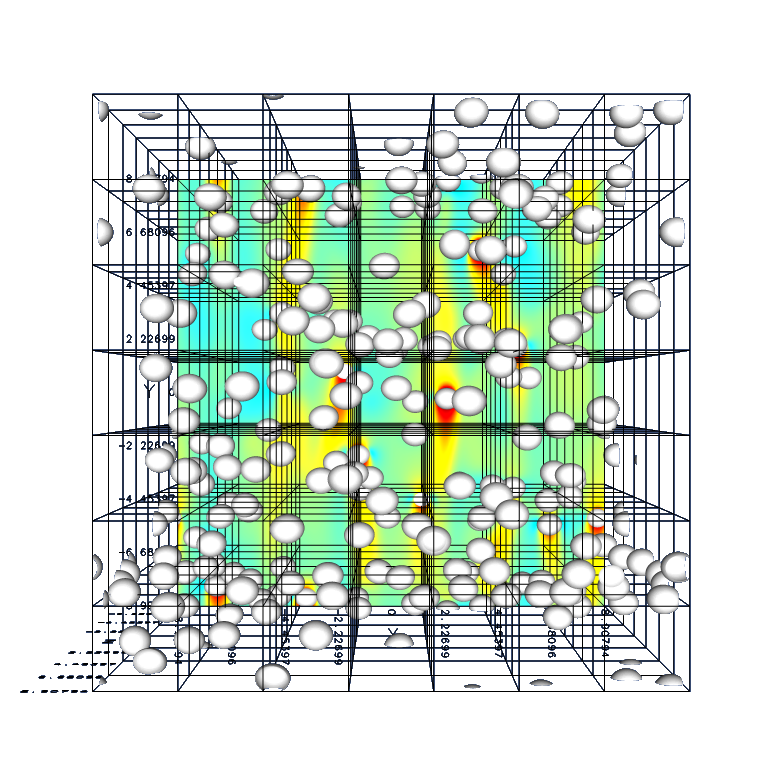
\includegraphics[width =  1.1\textwidth]{image/PHI_01_Ga_75.png}
\end{columns}
\end{frame}

\begin{frame}
  \frametitle{Direct Numerical Simulation of buoyant emulsions}
  \begin{columns}
    \column{0.6\textwidth}
  \underline{Dimensionless parameters :} 
  \begin{itemize}
    \item \textit{Galileo} number : $Ga =\frac{\sqrt{\rho \Delta\rho gD^3}}{\mu} \in [5, 100]$
    \item \textit{Bond} number : $Bo = \frac{\Delta \rho g D^2}{\sigma} = 1$ 
    \item volume fraction of dispersed phase : $\phi = [0.01;0.15]$. 
    \item Density and viscosity ratio, $\rho_r=1.11$ and $\mu_r= 0.1$. 
  \end{itemize}
  
  \begin{figure}
    \caption{Snapshot of a simulation at $T_g = 300$ for $\phi = 0.01$, $Ga = 75$ $\mu_r = 0.1$ and $N_b = 125$. In white : the interfaces, The background color map correspond to the pressure field. The grid represents the different core ($\le 729$ !).
    }
  \end{figure}
  \column{0.5\textwidth}
  \centering
  \href{file:///work/fintzin/BUBLLES_PROJECT/movies/cut.gif}{\beamergotobutton{Play}}
  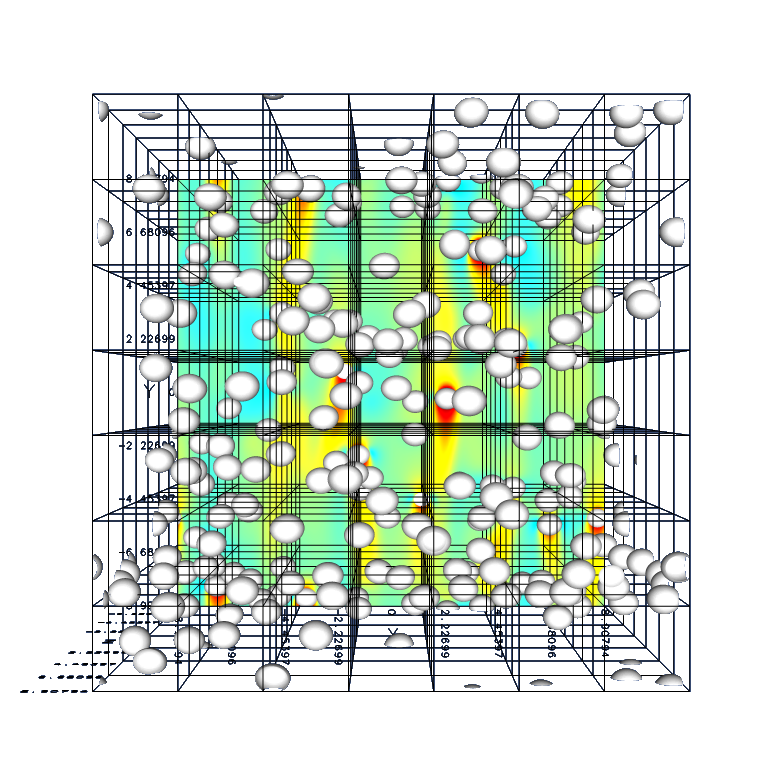
\includegraphics[width =  1.1\textwidth]{image/PHI_01_Ga_75.png}
  \end{columns}
\end{frame}

\begin{frame}
  \frametitle{Nearest pair probability density function}

  \begin{columns}
    \column{0.7\textwidth}
    \centering
    \begin{tabular}{cccc}
      &
      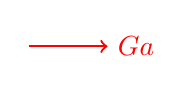
\begin{tikzpicture}[color=red]
        \draw[thick,->] (0,0) -- (1,0)node[right]{$Ga$};
      \end{tikzpicture}& & \\ 
        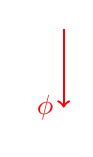
\begin{tikzpicture}[color=red]
          \draw[thick,->] (0,0) -- (0,-1)node[left]{$\phi$};
        \end{tikzpicture} &
        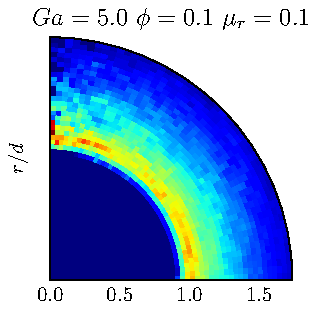
\includegraphics[height=0.3\textwidth]{image/HOMOGENEOUS/fDrop/Pnst_mu_r_0_1_Ga_5_PHI_0_1.pdf}  &
        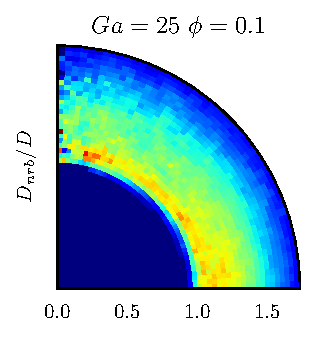
\includegraphics[height=0.3\textwidth]{image/HOMOGENEOUS/fDrop/Pnst_mu_r_0_1_Ga_25_PHI_0_1.pdf} &
        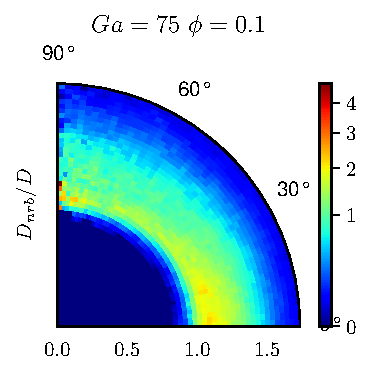
\includegraphics[height=0.3\textwidth]{image/HOMOGENEOUS/fDrop/Pnst_mu_r_0_1_Ga_75_PHI_0_1.pdf} 
        \\
         &
          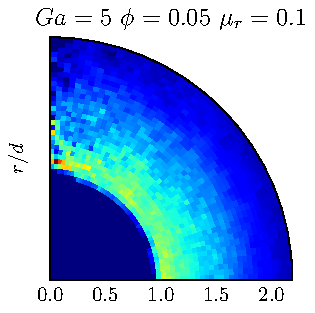
\includegraphics[height=0.3\textwidth]{image/HOMOGENEOUS/fDrop/Pnst_mu_r_0_1_Ga_5_PHI_0_05.pdf} &
        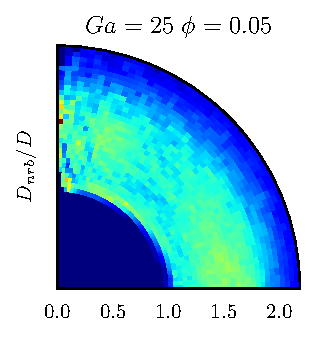
\includegraphics[height=0.3\textwidth]{image/HOMOGENEOUS/fDrop/Pnst_mu_r_0_1_Ga_25_PHI_0_05.pdf}&
        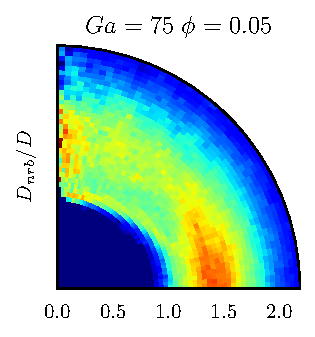
\includegraphics[height=0.3\textwidth]{image/HOMOGENEOUS/fDrop/Pnst_mu_r_0_1_Ga_75_PHI_0_05.pdf}\\
      \end{tabular}

      \column{0.3\textwidth}
      \begin{figure}
        \caption{Plots of $P_{nst} (\textbf{r})$ for different $Ga$ and $\phi$.}
      \end{figure}
    
    \begin{itemize}
      \item Drafting -Kissing tumbling mechanism for low $\phi$ and high $Ga$. 
    \end{itemize}
  \end{columns}
\end{frame}

\begin{frame}
  \frametitle{Reconstruction of the nearest relative velocity fields}

  \begin{figure}
    
    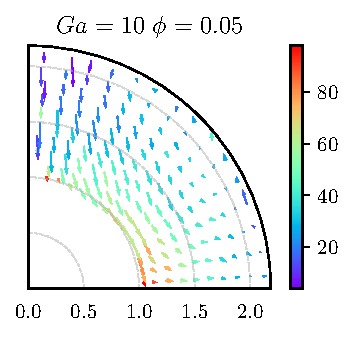
\includegraphics[height=0.25\textwidth]{image/HOMOGENEOUS/fDrop/U_mu_r_0_1_Ga_10_PHI_0_05.pdf}
    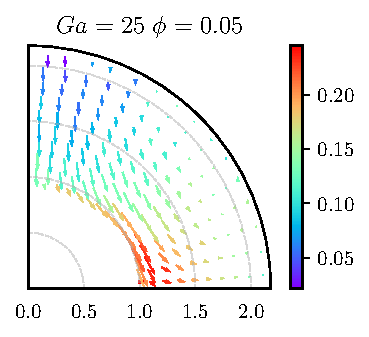
\includegraphics[height=0.25\textwidth]{image/HOMOGENEOUS/fDrop/U_mu_r_0_1_Ga_25_PHI_0_05.pdf}
    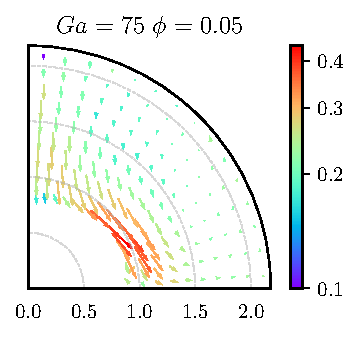
\includegraphics[height=0.25\textwidth]{image/HOMOGENEOUS/fDrop/U_mu_r_0_1_Ga_75_PHI_0_05.pdf}
    
    \caption{Nearest averaged velocity fields, $\nstrelavg{\textbf{u}} (\textbf{r})$ for different $Ga$ and $\phi$. 
    Colormap : magnitude of the relative velocity $|\nstrelavg{\textbf{u}}|$. }
  \end{figure}

\begin{itemize}
  \item In average particles approach from the top and leave through the sides. 
  % \item It is, again, a direct representation of the Drafting -Kissing tumbling mechanism since the velocity fields converge toward high density zone. 
\end{itemize}
\end{frame}



\begin{frame}
  \frametitle{Representation of the interaction force}

  \begin{figure}
    
    % 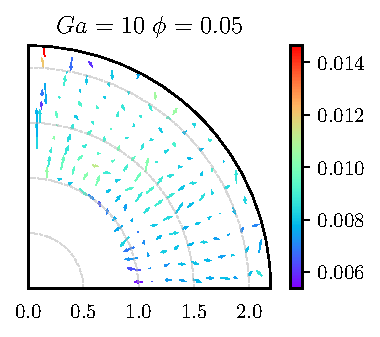
\includegraphics[height=0.25\textwidth]{image/HOMOGENEOUS/fDrop/F_mu_r_0_1_Ga_10_PHI_0_05.pdf}
    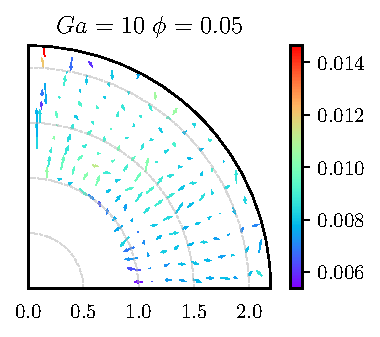
\includegraphics[height=0.25\textwidth]{image/HOMOGENEOUS/fDrop/F_mu_r_0_1_Ga_10_PHI_0_05.pdf}
    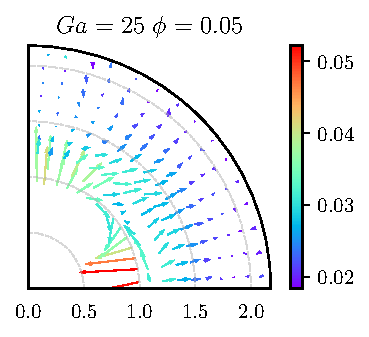
\includegraphics[height=0.25\textwidth]{image/HOMOGENEOUS/fDrop/F_mu_r_0_1_Ga_25_PHI_0_05.pdf}
    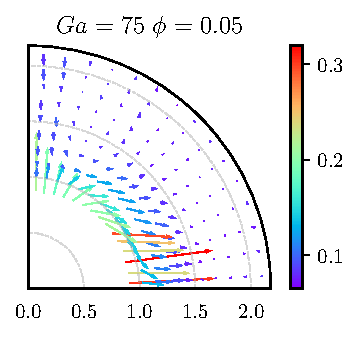
\includegraphics[height=0.25\textwidth]{image/HOMOGENEOUS/fDrop/F_mu_r_0_1_Ga_75_PHI_0_05.pdf}
    
    \caption{Nearest averaged relative acceleration fields times the mass of a particle. 
    Color map : Magnitude of the dimensionless force  $\nstrelavg{\textbf{F}} / (\Delta \rho V g)$.}
  \end{figure}

  
\begin{itemize}
  \item $\nstrelavg{\textbf{F}}$ is an isotropic repulsion force at high $Ga$. 
  \item At lower $Ga$ we observe attraction forces $\nstrelavg{\textbf{F}}$ on the sides.
\end{itemize}
\end{frame}

\begin{frame}
  \frametitle{Representation of the interaction force}

  \begin{figure}
    
    % 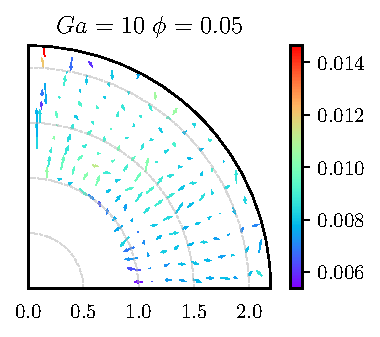
\includegraphics[height=0.25\textwidth]{image/HOMOGENEOUS/fDrop/F_mu_r_0_1_Ga_10_PHI_0_05.pdf}
    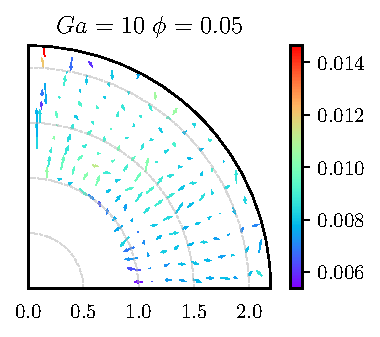
\includegraphics[height=0.25\textwidth]{image/HOMOGENEOUS/fDrop/F_mu_r_0_1_Ga_10_PHI_0_05.pdf}
    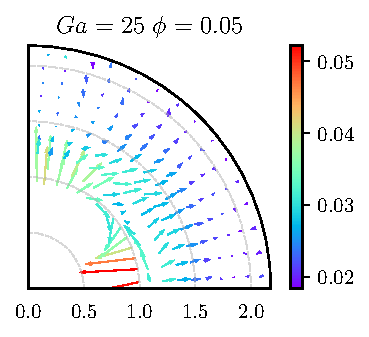
\includegraphics[height=0.25\textwidth]{image/HOMOGENEOUS/fDrop/F_mu_r_0_1_Ga_25_PHI_0_05.pdf}
    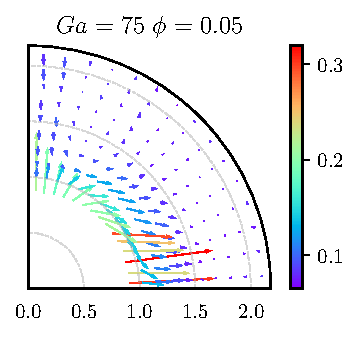
\includegraphics[height=0.25\textwidth]{image/HOMOGENEOUS/fDrop/F_mu_r_0_1_Ga_75_PHI_0_05.pdf}
    
    \caption{Nearest averaged relative acceleration fields times the mass of a particle. 
    Color map : Magnitude of the dimensionless force  $\nstrelavg{\textbf{F}} / (\Delta \rho V g)$.}
  \end{figure}

  
\begin{itemize}
  \item At low $Ga$ the magnitude of the force isn't correlated with \textbf{r}.
  \begin{itemize}
    \item Thus the relative hydrodynamic interactions are of the same order as the magnitude of the inter-particular interactions. 
  \end{itemize}
  \item  Visual representation of the particle stress : 
    $\bm{\Sigma}_{\text{PFP}} = \sum \textbf{r} 
    \nstavg{\textbf{F}}(\textbf{r}) 
    $
\end{itemize}
\end{frame}

\section{Coalescence modeling}

\begin{frame}
  \frametitle{Film drainage models to predict coalescence.}
  \begin{columns}
    \column{0.3\textwidth}
    \centering
    \begin{figure} 
      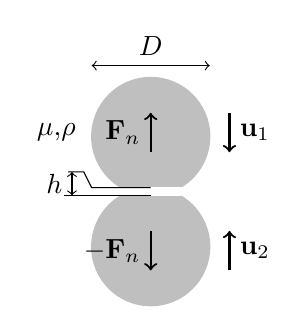
\begin{tikzpicture}
        \draw[lightgray,fill = lightgray] (0,0.7) circle (0.75);
        \draw[lightgray,fill = lightgray] (0,-0.7) circle (0.75);
        \draw[white,fill=white] (-0.75,-0.05) rectangle (0.75,0.05);
        \draw(0,0.05)--++(-0.75,0)--++(-0.1,0.2)--++(-0.2,0);
        \draw(0,-0.05)--++(-1.1,0);
        \draw[<->](-1,-0.05) --++ (0,0.3)node[midway,left]{$h$};
        \draw[<->](-0.75,1.6)--++(1.5,0)node[midway,above]{$D$};
        \node (para) at (-1.2,0.75){$\mu$,$\rho$};
        \draw[->,thick](0,0.5)--++(0,0.5)node[midway,left]{$\textbf{F}_n$};
        \draw[->,thick](0,-0.5)--++(0,-0.5)node[midway,left]{$-\textbf{F}_n$};
        \draw[<-,thick](1,0.5)--++(0,0.5)node[midway,right]{$\textbf{u}_1$};
        \draw[<-,thick](1,-0.5)--++(0,-0.5)node[midway,right]{$\textbf{u}_2$};
      \end{tikzpicture}
      \caption{Scheme of two colliding droplets.}
    \end{figure}
    \column{0.7\textwidth}
    \begin{columns}[t]
      \column{0.5\textwidth}
      \textbf{Current film thickness : }  
      \begin{equation*}
        \frac{h(t_c,F_n)}{D}  \sim \frac{F_n \mu^{1/2}}{t_c \sigma} 
      \end{equation*}
      \begin{itemize}
        \item \underline{$F_n$ : Interaction force}
        \item $D$ : Droplets diameters
        \item $\sigma$ : Surface tension coefficient
        \item \underline{$t_c$ : contact time}
      \end{itemize}
      \citet{chesters1991modelling}
      \column{0.5\textwidth}
      \textbf{Critical thickness \footnote{\citet{yoon2007coalescence}}} 
      \begin{equation*}
        \frac{h_c}{D} \sim  \frac{A_HCa^{1/6}}{\sigma^{1/3}} 
      \end{equation*}
      \begin{itemize}
        \item $Ca$ : Capillary number 
        \item $A_H = 2.4\cdot 10^{-21}$ : Hamaker constant
      \end{itemize}
    \end{columns}
  \end{columns}
  \vfill
  \begin{itemize}
    \item How to estimate $F_n$ and $t_c$ ? 
  \end{itemize}
\end{frame}

\begin{frame}
  \frametitle{Prediction of $F_n$ and $t_c$ with DNS results.}
  \begin{columns}
    \column{0.3\textwidth}
    \centering
    \begin{figure} 
      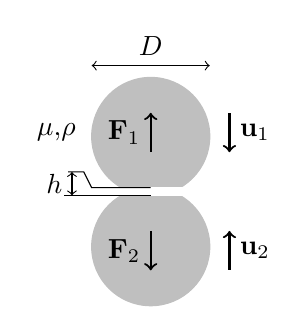
\begin{tikzpicture}
        \draw[lightgray,fill = lightgray] (0,0.7) circle (0.75);
        \draw[lightgray,fill = lightgray] (0,-0.7) circle (0.75);
        \draw[white,fill=white] (-0.75,-0.05) rectangle (0.75,0.05);
        \draw(0,0.05)--++(-0.75,0)--++(-0.1,0.2)--++(-0.2,0);
        \draw(0,-0.05)--++(-1.1,0);
        \draw[<->](-1,-0.05) --++ (0,0.3)node[midway,left]{$h$};
        \draw[<->](-0.75,1.6)--++(1.5,0)node[midway,above]{$D$};
        \node (para) at (-1.2,0.75){$\mu$,$\rho$};
        \draw[->,thick](0,0.5)--++(0,0.5)node[midway,left]{$\textbf{F}_1$};
        \draw[->,thick](0,-0.5)--++(0,-0.5)node[midway,left]{$\textbf{F}_2$};
        \draw[<-,thick](1,0.5)--++(0,0.5)node[midway,right]{$\textbf{u}_1$};
        \draw[<-,thick](1,-0.5)--++(0,-0.5)node[midway,right]{$\textbf{u}_2$};
      \end{tikzpicture}
      \caption{Scheme of two colliding droplets labeled $1$ and $2$.}
    \end{figure}
    \column{0.7\textwidth}
    \begin{columns}
      \column{0.5\textwidth}
      \centering
      \begin{figure}
        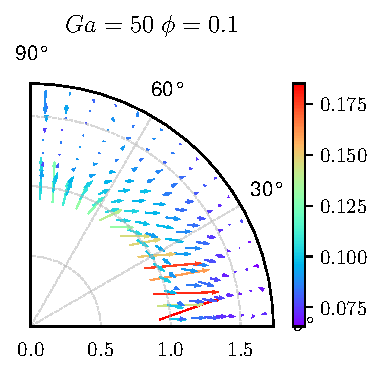
\includegraphics[width=0.9\textwidth]{image/HOMOGENEOUS/fDrop/F_mu_r_0_1_Ga_50_PHI_0_1.pdf}
        \caption{Nearest relative averaged force fields, $\nstrelavg{\textbf{F}}(\textbf{r})$.}
      \end{figure}
      \column{0.5\textwidth}
      \centering
      \begin{figure}
      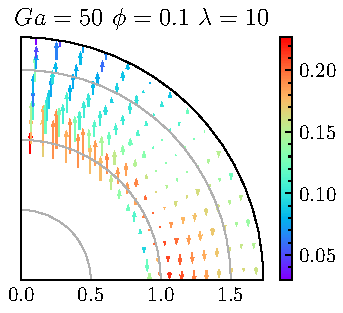
\includegraphics[width=0.9\textwidth]{image/HOMOGENEOUS/fDrop/U_mu_r_0_1_Ga_50_PHI_0_1.pdf}
      \caption{Relative averaged velocity fields, $\nstrelavg{\textbf{u}}(\textbf{r})$.}
    \end{figure}
    \end{columns}
  \end{columns}
  \begin{itemize}
    \item We notice that $F_c$ and $t_c$ are function of \textbf{r}, $\phi$, $Ga$, $\mu_r$ \ldots
    \item Therefore,
    $ h(t_c,F_n)  \sim F_n(\textbf{r}) / t_c(\textbf{r}) D \sigma^{-1} \mu^{1/2}$
  \end{itemize}
\end{frame}

\begin{frame}
  \frametitle{Motion and coalesce of the nearest droplet}
\centering
\begin{tikzpicture}
  \node (img) at (0,0) {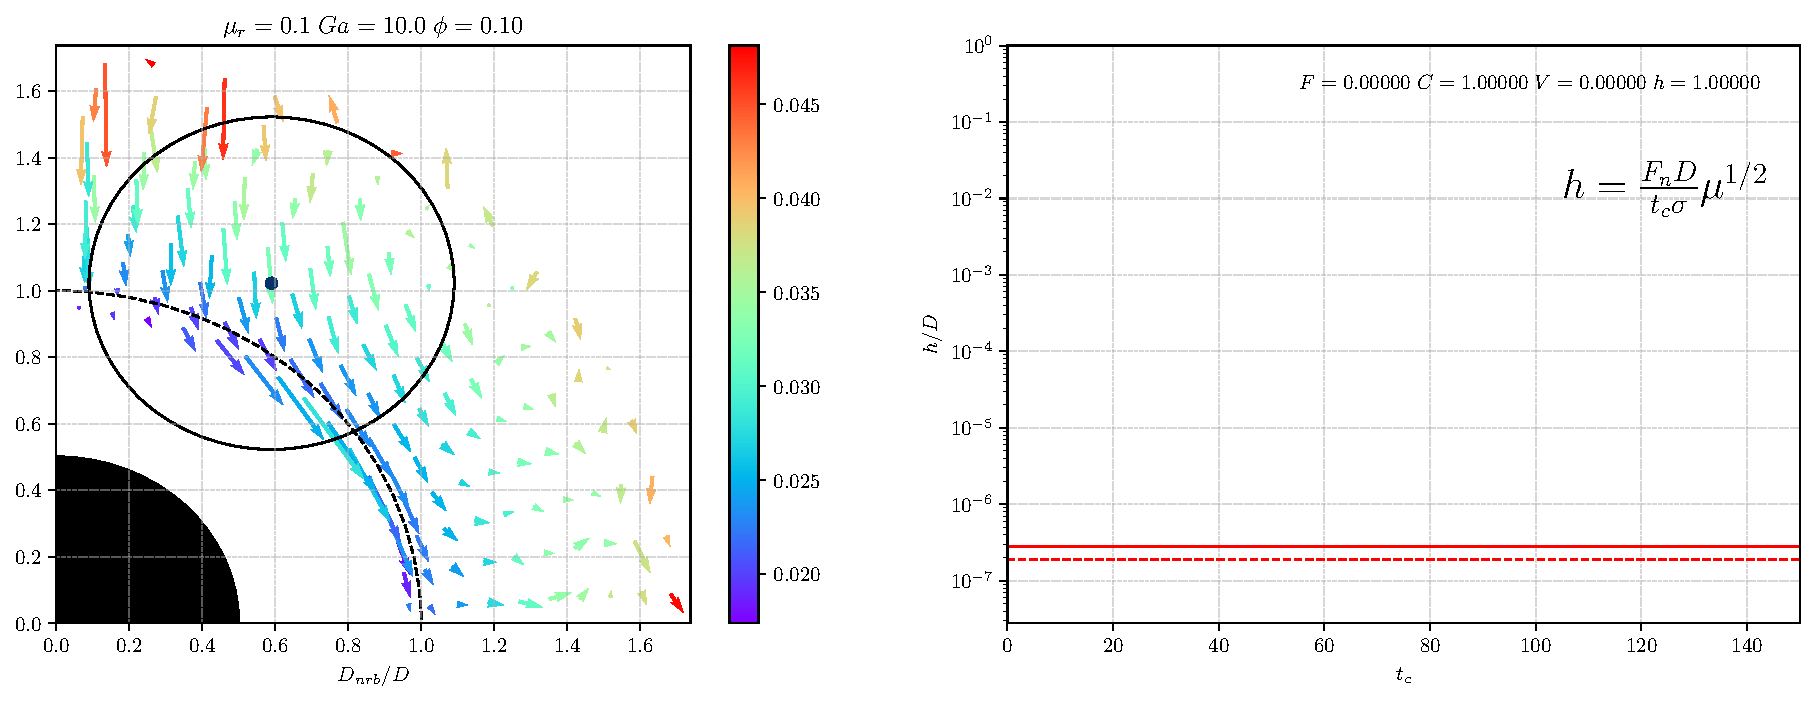
\includegraphics[width=\textwidth]{image/HOMOGENEOUS/anim/frame_1_0_1_Ga_10_PHI_0_1.pdf}};
  \node (hc) at (1.4,-1.8) {\textcolor{red}{$h_c$}};
\end{tikzpicture}
  % \includegraphics[width=\textwidth]{../movies/P_PHI_1_Ga_75.gif}
  
  $Ga = 10$ :
  \href{file:///work/fintzin/BUBLLES_PROJECT/movies/First_anim.mp4}{\beamergotobutton{Play}}\\
  $Ga = 25$ :
  \href{file:///work/fintzin/BUBLLES_PROJECT/results/HOMOGENEOUS/Dim_3/N_5/PHI_0.1/rho_r_1.11/Bo_1/mu_r_0.1/Ga_25/animation_N1.mp4}{\beamergotobutton{Play}}\\
  $Ga = 50$ :
  \href{file:///work/fintzin/BUBLLES_PROJECT/results/HOMOGENEOUS/Dim_3/N_5/PHI_0.1/rho_r_1.11/Bo_1/mu_r_0.1/Ga_50/animation_N1.mp4}{\beamergotobutton{Play}}
\end{frame}

\begin{frame}
  \frametitle{Motion and coalesce of the nearest droplets }
\centering
  \begin{tikzpicture}
    \node (img) at (0,0) {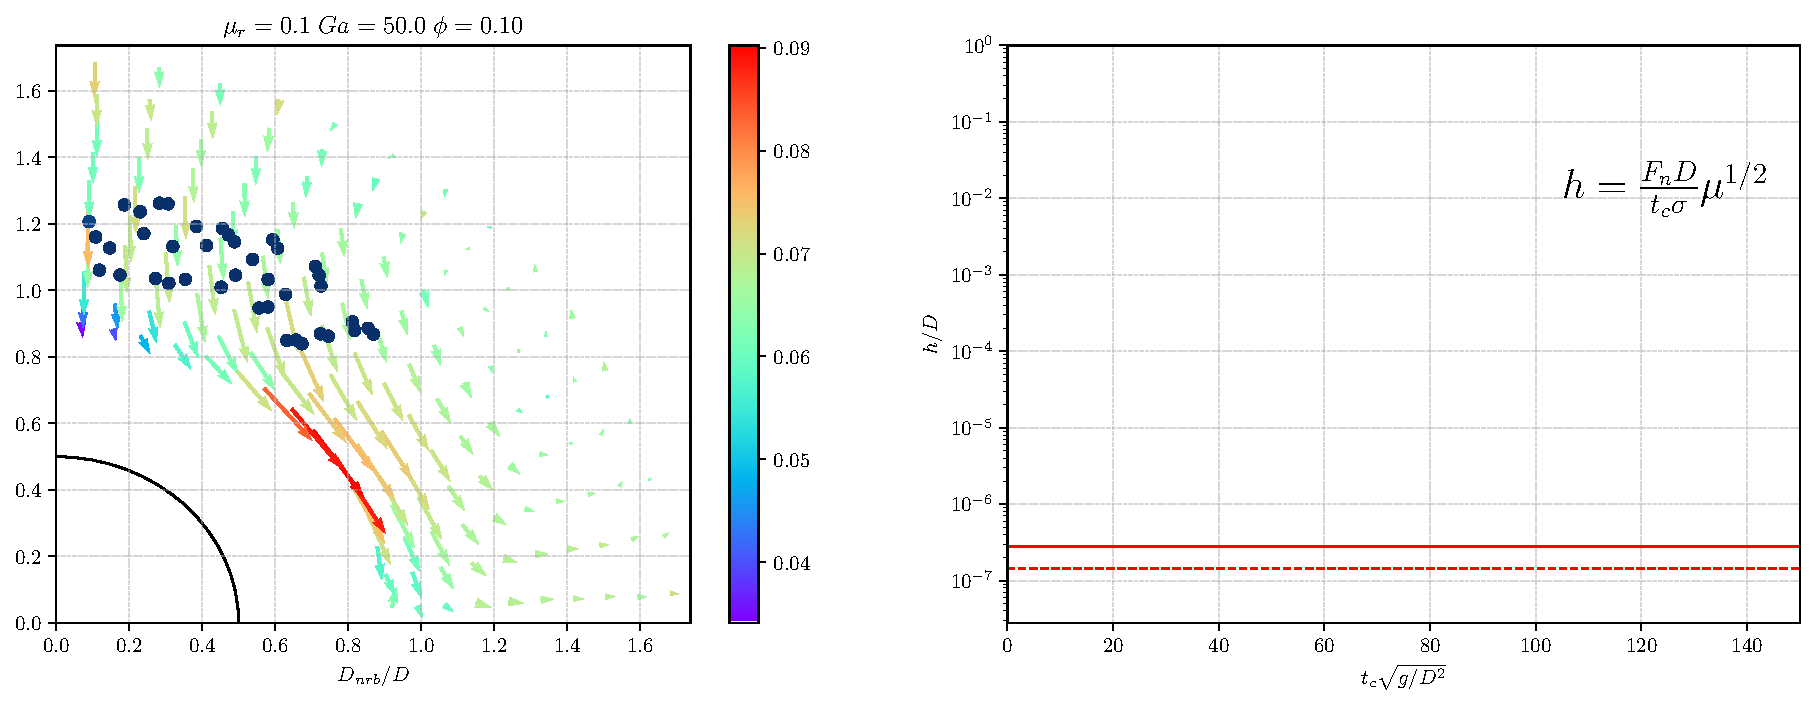
\includegraphics[width=\textwidth]{image/HOMOGENEOUS/anim/frame_1_N40_0_1_Ga_50_PHI_0_1.pdf}};
    \node (hc) at (1.4,-1.8) {\textcolor{red}{$h_c$}};
  \end{tikzpicture}
  % \href{file:///work/fintzin/BUBLLES_PROJECT/results/HOMOGENEOUS/Dim_3/N_5/PHI_0.1/rho_r_1.11/Bo_1/mu_r_0.1/Ga_25/animation_N1.mp4}{\beamergotobutton{Play}}
  
  \begin{columns}
    \column{0.5\textwidth}
    \centering
    \begin{tabular}{|c|c|c|}\hline
       &
      $Ga = 10$ &
      \href{file:///work/fintzin/BUBLLES_PROJECT/results/HOMOGENEOUS/Dim_3/N_5/PHI_0.1/rho_r_1.11/Bo_1/mu_r_0.1/Ga_10/animation.mp4}{\beamergotobutton{Play}}\\
      $\phi = 0.1$&
      $Ga = 25$ &
      \href{file:///work/fintzin/BUBLLES_PROJECT/results/HOMOGENEOUS/Dim_3/N_5/PHI_0.1/rho_r_1.11/Bo_1/mu_r_0.1/Ga_25/animation.mp4}{\beamergotobutton{Play}}\\
      &
      $Ga = 50$ &
      \href{file:///work/fintzin/BUBLLES_PROJECT/results/HOMOGENEOUS/Dim_3/N_5/PHI_0.1/rho_r_1.11/Bo_1/mu_r_0.1/Ga_50/animation.mp4}{\beamergotobutton{Play}}\\\hline
    \end{tabular}
    \column{0.5\textwidth}
    \centering
    \begin{tabular}{|c|c|c|}\hline
      &
     $Ga = 10$ &
     \href{file:///work/fintzin/BUBLLES_PROJECT/results/HOMOGENEOUS/Dim_3/N_5/PHI_0.01/rho_r_1.11/Bo_1/mu_r_0.1/Ga_10/animation.mp4}{\beamergotobutton{Play}}\\
     $\phi = 0.01$&
     $Ga = 25$ &
     \href{file:///work/fintzin/BUBLLES_PROJECT/results/HOMOGENEOUS/Dim_3/N_5/PHI_0.01/rho_r_1.11/Bo_1/mu_r_0.1/Ga_25/animation.mp4}{\beamergotobutton{Play}}\\
     &
     $Ga = 50$ &
     \href{file:///work/fintzin/BUBLLES_PROJECT/results/HOMOGENEOUS/Dim_3/N_5/PHI_0.01/rho_r_1.11/Bo_1/mu_r_0.1/Ga_50/animation.mp4}{\beamergotobutton{Play}}\\\hline
   \end{tabular}
  \end{columns}
\end{frame}

\section{Conclusion and discussion}
\begin{frame}
  \frametitle{General remarks and conclusion}

  \begin{itemize}
    \item We used the nearest particle statistics to describe pair interactions in oil/water emulsion. 
    \item The relative velocity, and forces/acceleration are directly correlated to the relative position, $Ga$ and $\phi$. 
    \item We predicted coalesce event in the different regime. 
  \end{itemize}
  Future projects :   
  \begin{itemize}
    \item Deriving semi empirical formulation for the coalescence source term $\avg{S}$, which takes in account the phenomenology of interactions in emulsion presented in this work. 
  \end{itemize}

\vspace{1cm}
\textbf{The buoyant emulsion DNS code is open source and available at} : 
\url{http://basilisk.fr/sandbox/fintzin/Rising-Suspenion/}
\end{frame}

\begin{frame}
  \frametitle{Other correlations for the averaged Navier Stokes equations}
\begin{columns}
  \begin{column}{0.5\textwidth}
    \begin{figure}
      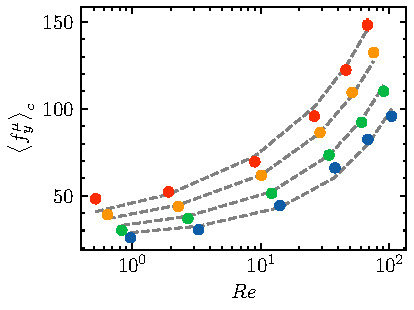
\includegraphics[width=0.7\textwidth]{image/HOMOGENEOUS/fCA/FH_mu_Re.pdf}
      \caption{Dimensionless drag force in terms $Re$ for $\phi = 0.01, 0.05, 0.1$ and $0.15$.}
    \end{figure}
    \begin{equation*}
      \frac{\avg{f}}{\mu UD} 
      = 1.18 e^{5.32\phi^{1/3}}  Re^{0.33}  + Re^{0.87} +24.12
    \end{equation*}
  \end{column}
  \begin{column}{0.5\textwidth}
    \begin{figure}[h!]
      \centering
      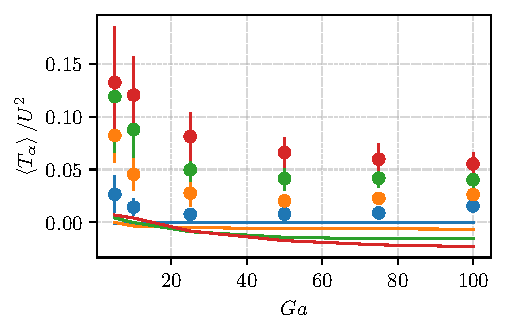
\includegraphics[width=0.7\textwidth]{image/HOMOGENEOUS/fPA/Talpha.pdf}
      \caption{Dimensionless granular temperature in terms of $Ga$ and $\phi$}
  \end{figure}
  	\begin{equation}
    \frac{\avg{\textbf{u}'\cdot \textbf{u}'}}{U^2}  
    \approx \frac{\phi}{Ga^2} 2.86\cdot10^{4} 
    \label{eq:Talpha_scaling}
	\end{equation}
    % \begin{itemize}
    %   \item $U$ is the relative velocity between the continuous and dispersed phase.
    %   \item $Re$ is the \textit{Reynolds} number defined as, $Re = \rho D U / \mu$. 
    % \end{itemize}
  \end{column}
\end{columns}
\end{frame}


\begin{frame}[t]
  \frametitle{References}
  \bibliography{Bib/bib_bulles.bib}
\end{frame}

 
\backmatter
\begin{frame}
  \frametitle{Computation of the damping ratio ? }
  \begin{figure}
    \centering
    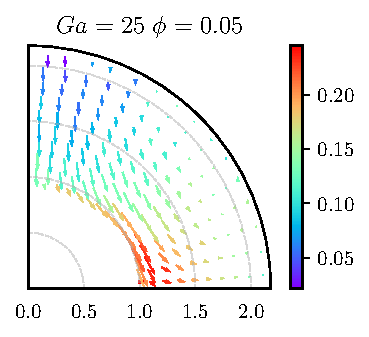
\includegraphics[width=0.27\textwidth]{image/HOMOGENEOUS/fDrop/U_mu_r_0_1_Ga_25_PHI_0_05.pdf}
    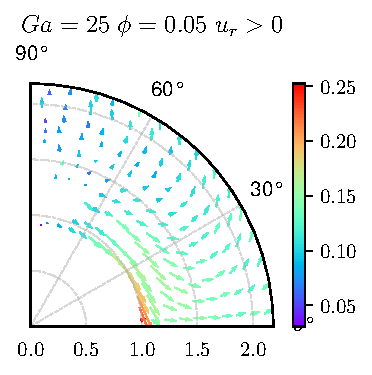
\includegraphics[width=0.27\textwidth]{image/HOMOGENEOUS/fDrop/Upos_mu_r_0_1_Ga_25_PHI_0_05.pdf}
    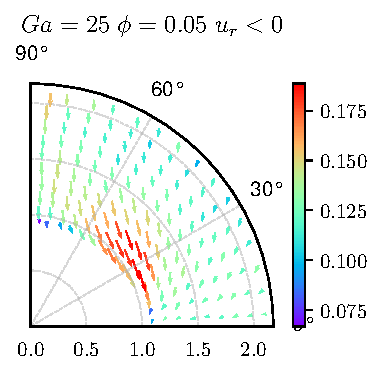
\includegraphics[width=0.27\textwidth]{image/HOMOGENEOUS/fDrop/Uneg_mu_r_0_1_Ga_25_PHI_0_05.pdf}
    \caption{Nearest averaged force fields, $\nstrelavg{\textbf{u}}(\textbf{r})$ for different $Ga$ and $\phi$. 
    Color map : Magnitude of the dimensionless force  $\nstrelavg{\textbf{u}} / (\Delta \rho V g)$.
    (middle) conditional average  $\nstrelavg{\textbf{u}| u_r > 0}(\textbf{r})$. 
    (right) conditional average  $\nstrelavg{\textbf{u}| u_r < 0}(\textbf{r})$ }
  \end{figure}
  \begin{equation}
    \text{Damping Ratio}
    \approx \frac{\avg{\frac{1}{2} \textbf{u} \cdot \textbf{u}| u_r > 0}}
    {\avg{\frac{1}{2}\textbf{u}\cdot \textbf{u}| u_r < 0}}
    = 0.12
  \end{equation}
\end{frame}

\begin{frame}
  \frametitle{Conditional average of the force on the velocity}
  \begin{figure}
    \centering
    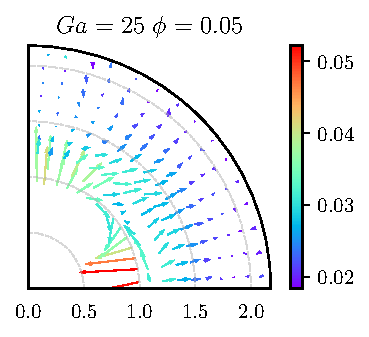
\includegraphics[width=0.33\textwidth]{image/HOMOGENEOUS/fDrop/F_mu_r_0_1_Ga_25_PHI_0_05.pdf}
    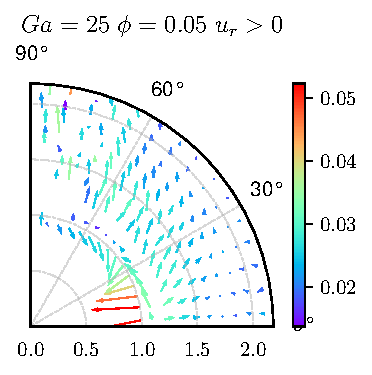
\includegraphics[width=0.33\textwidth]{image/HOMOGENEOUS/fDrop/Fpos_mu_r_0_1_Ga_25_PHI_0_05.pdf}
    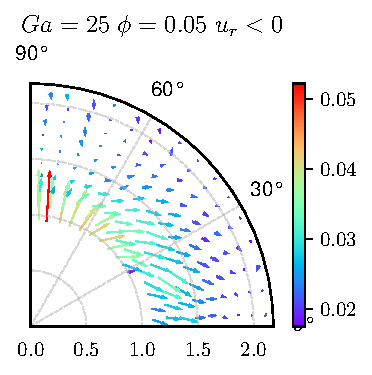
\includegraphics[width=0.33\textwidth]{image/HOMOGENEOUS/fDrop/Fneg_mu_r_0_1_Ga_25_PHI_0_05.pdf}
    \caption{Nearest averaged force fields, $\nstrelavg{\textbf{F}}(\textbf{r})$ for different $Ga$ and $\phi$. 
    Color map : Magnitude of the dimensionless force  $\nstrelavg{\textbf{F}} / (\Delta \rho V g)$.
    (middle) conditional average  $\nstrelavg{\textbf{F}| u_r > 0}(\textbf{r})$. 
    (right) conditional average  $\nstrelavg{\textbf{F}| u_r < 0}(\textbf{r})$ }
  \end{figure}
\end{frame}

\begin{frame}
  \frametitle{Conditional average of the force on the velocity}
  \begin{figure}
    \centering
    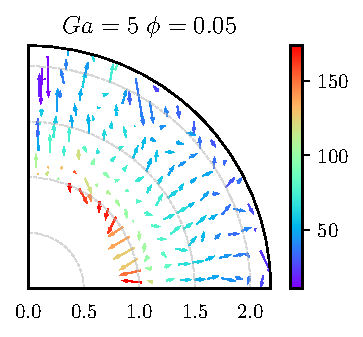
\includegraphics[width=0.33\textwidth]{image/HOMOGENEOUS/fDrop/F_mu_r_0_1_Ga_5_PHI_0_05.pdf}
    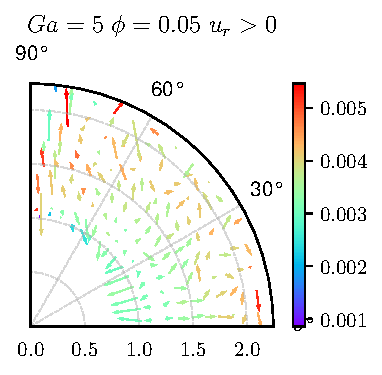
\includegraphics[width=0.33\textwidth]{image/HOMOGENEOUS/fDrop/Fpos_mu_r_0_1_Ga_5_PHI_0_05.pdf}
    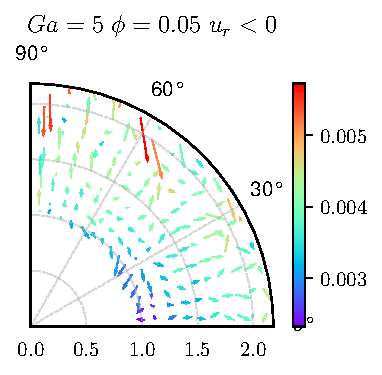
\includegraphics[width=0.33\textwidth]{image/HOMOGENEOUS/fDrop/Fneg_mu_r_0_1_Ga_5_PHI_0_05.pdf}
    \caption{Nearest averaged force fields, $\nstrelavg{\textbf{F}}(\textbf{r})$ for different $Ga$ and $\phi$. 
    Color map : Magnitude of the dimensionless force  $\nstrelavg{\textbf{F}} / (\Delta \rho V g)$.
    (middle) conditional average  $\nstrelavg{\textbf{F}| u_r > 0}(\textbf{r})$. 
    (right) conditional average  $\nstrelavg{\textbf{F}| u_r < 0}(\textbf{r})$ }
  \end{figure}
\end{frame}


  
\end{document}
